% Midterm presentation. Build: cd docs/slides/midterm && latexmk -xelatex midterm.tex
\documentclass[aspectratio=169,12pt]{beamer}
\usepackage{fontspec}
\usepackage[ukrainian]{babel}
\setsansfont{Lato}[BoldFont=Lato Bold]
\setmainfont{Lato}[BoldFont=Lato Bold]
\setmonofont{DejaVu Sans Mono}[Scale=0.8]
\newfontfamily\symbolfont{DejaVu Sans}
\usepackage{booktabs}
\usepackage{tikz}
\usetikzlibrary{arrows.meta,positioning}

% --- look: white slides, big thin centred titles, turquoise blocks ------------
\definecolor{ink}{HTML}{0F1F1E}
\definecolor{teal}{HTML}{0D9488}
\definecolor{tealdark}{HTML}{0F766E}
\definecolor{aqua}{HTML}{A7F3EB}
\definecolor{aqualight}{HTML}{E6FBF8}
\definecolor{muted}{HTML}{7A8A89}
\definecolor{metal}{HTML}{3B82F6}
\definecolor{plastic}{HTML}{F59E0B}
\definecolor{warn}{HTML}{E5484D}
\definecolor{good}{HTML}{0D9488}
\setbeamercolor{normal text}{fg=ink,bg=white}
\setbeamercolor{frametitle}{fg=ink}
\setbeamercolor{structure}{fg=teal}
\setbeamerfont{frametitle}{size=\LARGE}
\setbeamertemplate{frametitle}{\vspace*{0.9em}\centering\insertframetitle\par}
\setbeamertemplate{navigation symbols}{}
\setbeamertemplate{itemize items}{\color{teal}\textbullet}
\setbeamertemplate{footline}{\hfill{\color{muted}\scriptsize\insertframenumber}\hspace*{1.2em}\vspace*{0.7em}}
\setlength{\leftmargini}{1.2em}
\hyphenpenalty=10000 \exhyphenpenalty=10000

\tikzset{
  blk/.style={fill=teal, text=white, rounded corners=4pt, minimum height=9mm, inner xsep=8pt, font=\small\bfseries, align=center},
  leaf/.style={fill=aqua, text=ink, rounded corners=4pt, minimum height=9mm, inner xsep=8pt, font=\small, align=center},
  pale/.style={fill=aqualight, text=muted, rounded corners=4pt, minimum height=9mm, inner xsep=8pt, font=\small, align=center},
  arr/.style={-{Stealth[length=2.4mm]}, line width=0.8pt, draw=ink},
}
\newcommand{\done}{{\color{good}\symbolfont ✓}}
\newcommand{\notdone}{{\color{warn}\symbolfont ✗}}
\newcommand{\bignum}[1]{{\fontsize{30}{32}\selectfont\bfseries\color{tealdark} #1}}

\begin{document}

% 1 ---------------------------------------------------------------------------
{
\setbeamertemplate{background}{\begin{tikzpicture}
  \shade[top color=aqua, bottom color=white, shading angle=-30] (0,0) rectangle (\paperwidth,\paperheight);
\end{tikzpicture}}
\setbeamertemplate{footline}{}
\begin{frame}
  \centering
  \vspace{2.2em}
  {\fontsize{46}{50}\selectfont Cleany}\\[0.5em]
  {\Large робот, що сортує сміття}\\[2.2em]
  {\large Єлизавета Бугір \quad·\quad Назар Пасічник}\\[0.6em]
  {\color{muted} Проміжний захист · 25 жовтня 2026}
\end{frame}
}

% 2 ---------------------------------------------------------------------------
\begin{frame}{Задача}
  \centering
  {\large Рука бачить предмет і кладе його в потрібний кошик}\\[0.6em]
  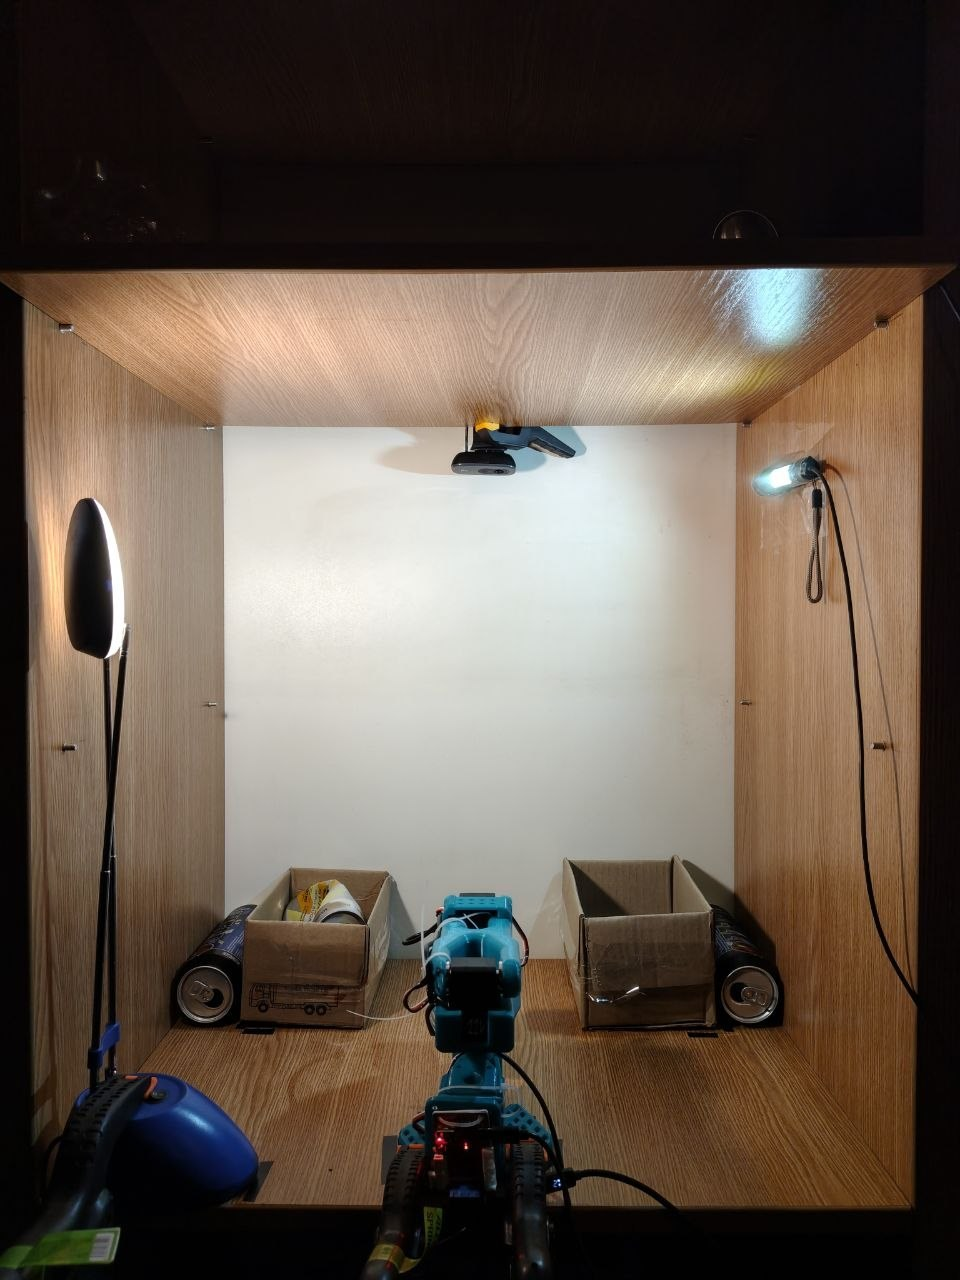
\includegraphics[height=0.52\textheight]{figures/setup_clean.jpg}\quad
  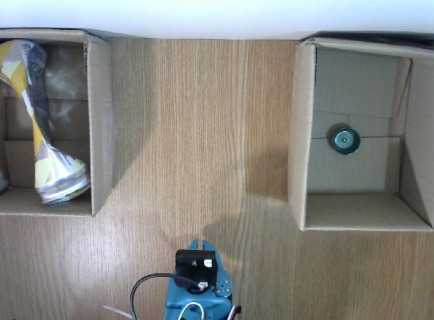
\includegraphics[height=0.52\textheight]{figures/front_view.jpg}\\[0.7em]
  \small
  \tikz[baseline=-0.6ex]\node[leaf, fill=metal!25]{метал $\to$ ліворуч}; \quad
  \tikz[baseline=-0.6ex]\node[leaf, fill=plastic!30]{пластик $\to$ праворуч}; \quad
  \tikz[baseline=-0.6ex]\node[pale]{інше $\to$ люк ESP32 (план)};
\end{frame}

% 3 ---------------------------------------------------------------------------
\begin{frame}{Pipeline зараз}
  \centering
  \vspace{1.5em}
  \begin{tikzpicture}[node distance=7mm and 8mm]
    \node[leaf] (cam) {Камера};
    \node[blk, right=of cam] (yolo) {YOLO};
    \node[blk, right=of yolo] (lock) {той самий клас\\$\geq T$ секунд?};
    \node[leaf, right=of lock, yshift=8mm, fill=metal!25] (am) {ACT метал};
    \node[leaf, right=of lock, yshift=-8mm, fill=plastic!30] (ap) {ACT пластик};
    \node[leaf, right=of am, yshift=-8mm] (home) {Додому};
    \draw[arr] (cam) -- (yolo);
    \draw[arr] (yolo) -- (lock);
    \draw[arr] (lock) -- (am.west);
    \draw[arr] (lock) -- (ap.west);
    \draw[arr] (am.east) -- (home);
    \draw[arr] (ap.east) -- (home);
    \draw[arr] (home.south) |- ++(0,-1.6) -| (cam.south);
  \end{tikzpicture}
  \vspace{2em}

  \color{muted}$T$ — поріг часу YOLO, напр. 3 с\\[0.3em]YOLO вирішує один раз · окрема ACT на кожен матеріал
\end{frame}

% 4 ---------------------------------------------------------------------------
\begin{frame}{Дані}
  \begin{columns}[c]
    \begin{column}{0.3\textwidth}
      \centering
      \bignum{140}\\демонстрацій\\[1em]
      \bignum{80k}\\кадрів, 30 fps\\[1em]
      \bignum{100}\\розмічених кадрів\\[1em]
      {\scriptsize\color{muted} усе записано нами\\Hugging Face Hub}
    \end{column}
    \begin{column}{0.66\textwidth}
      \centering
      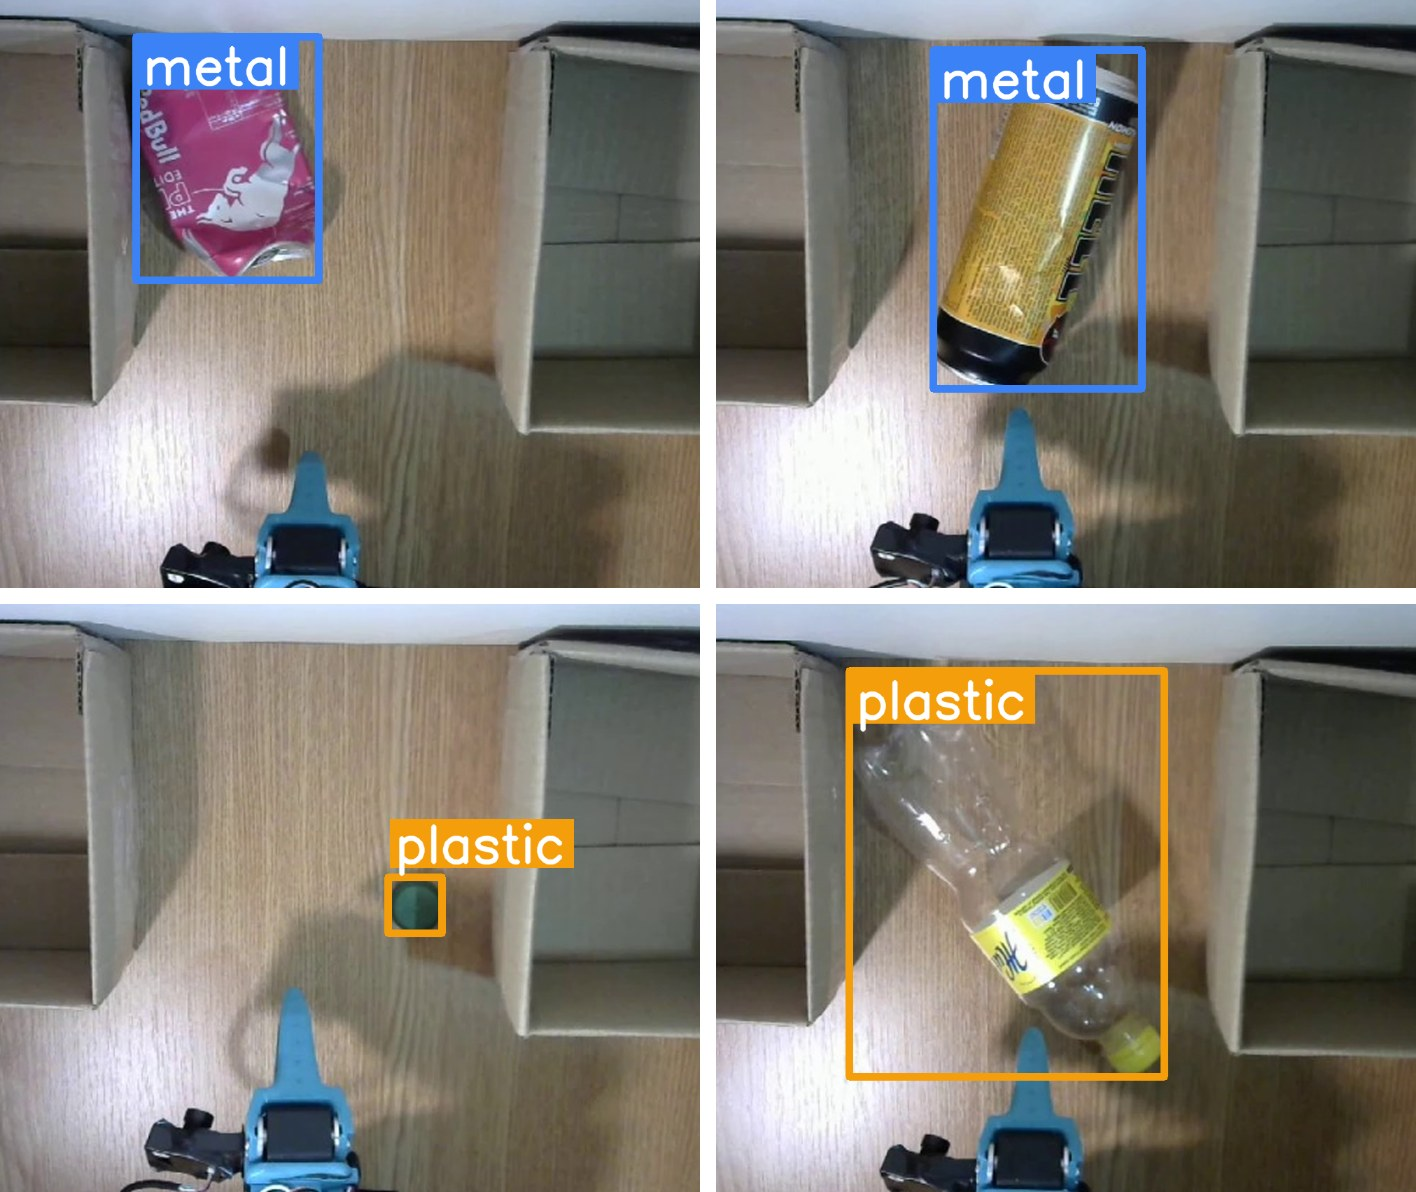
\includegraphics[height=0.8\textheight]{figures/frames_big.jpg}
    \end{column}
  \end{columns}
\end{frame}

% 5 ---------------------------------------------------------------------------
\begin{frame}{Baseline і метрики}
  \begin{columns}[c]
    \begin{column}{0.56\textwidth}
      \centering
      \begin{tabular}{@{}lcc@{}}
        \toprule
        YOLO & val & тест \\
        \midrule
        Baseline (Kaggle) & 0.002 & 0/8 \\
        \textbf{Наші кадри} & \textbf{0.870} & \textbf{8/8} \\
        + Kaggle & 0.869 & 6/8 \\
        Більша модель & 0.858 & 2 зайві \\
        \bottomrule
      \end{tabular}\\[0.5em]
      {\scriptsize\color{muted} val: mAP\textsubscript{50-95}, 20 кадрів · тест: фото з іншої камери}
      \vspace{1.2em}

      \small
      \tikz[baseline=-0.6ex]\node[blk]{ACT на руці: пластик 9/10 · метал 8/10};\\[0.4em]
      {\scriptsize\color{muted} 10 спроб на модель · 100k кроків кожна}
    \end{column}
    \begin{column}{0.42\textwidth}
      \centering
      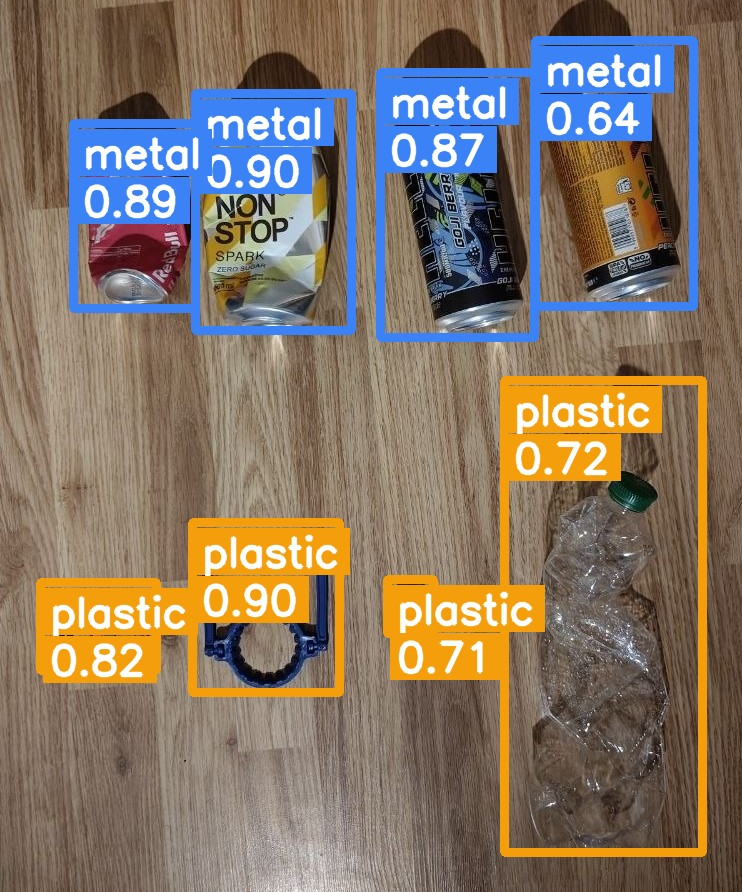
\includegraphics[height=0.74\textheight]{figures/yolo_test_ours.jpg}\\[0.1em]
      {\scriptsize\color{muted} наша модель на новому фото · baseline: 0 з 8}
    \end{column}
  \end{columns}
\end{frame}

% 6 ---------------------------------------------------------------------------
\begin{frame}{Прогрес}
  \begin{columns}[T]
    \begin{column}{0.48\textwidth}
      \large
      \done\ стенд і камери\\[0.15em]
      \done\ 140 демонстрацій\\[0.15em]
      \done\ YOLO на наших даних\\[0.15em]
      \done\ 2 ACT-моделі\\[0.15em]
      \done\ pipeline\\[0.15em]
      \done\ на руці: 9/10 і 8/10
    \end{column}
    \begin{column}{0.48\textwidth}
      \large
      \notdone\ клас «інше» + ESP32\\
      {\small\color{muted}\quad коробка ще не фінальна}\\[0.3em]
      \notdone\ SmolVLA\\
      {\small\color{muted}\quad не влазить у 4 ГБ GPU}
    \end{column}
  \end{columns}
  \vspace{0.6em}
  \centering\footnotesize
  \tikz[baseline=-0.6ex]\node[leaf]{\textbf{Назар}: стенд, камери, запис, тренування}; \quad
  \tikz[baseline=-0.6ex]\node[leaf]{\textbf{Єлизавета}: YOLO, ACT, pipeline};
\end{frame}

% 7 ---------------------------------------------------------------------------
\begin{frame}{Новий pipeline {\large\color{muted}(фіналізуємо)}}
  \centering
  \vspace{0.6em}
  \begin{tikzpicture}[node distance=6mm and 5mm, scale=0.9, transform shape]
    \node[leaf] (cam) {Камера};
    \node[blk, right=of cam] (yolo) {YOLO\\+ DINOv3};
    \node[blk, right=of yolo, fill=tealdark] (pick) {Одна модель\\«взяти»};
    \node[blk, right=of pick] (ok) {Захват\\вдався?};
    \node[leaf, right=of ok, yshift=8mm, fill=metal!25] (pm) {скрипт $\to$ метал};
    \node[leaf, right=of ok, yshift=-8mm, fill=plastic!30] (pp) {скрипт $\to$ пластик};
    \draw[arr] (cam) -- (yolo);
    \draw[arr] (yolo) -- (pick);
    \draw[arr] (pick) -- (ok);
    \draw[arr] (ok) -- (pm.west);
    \draw[arr] (ok) -- (pp.west);
    \draw[arr] (ok.south) -- ++(0,-0.9) -| node[pos=0.25, below, font=\scriptsize, text=muted] {ні — ще спроба} (pick.south);
  \end{tikzpicture}
  \vspace{1em}

  \begin{tikzpicture}[node distance=4mm, every node/.append style={font=\footnotesize}]
    \node[pale, text width=40mm, text=ink] (a) {\textbf{1 модель, 2× даних}\\140 епізодів до\\моменту «взяли»};
    \node[pale, text width=40mm, text=ink, right=of a] (b) {\textbf{«Покласти» без ML}\\пози над кошиками\\+ відкрити клешню};
    \node[pale, text width=40mm, text=ink, right=of b] (c) {\textbf{Захват — серво}\\позиція клешні\\+ навантаження};
  \end{tikzpicture}
\end{frame}

% 8 ---------------------------------------------------------------------------
\begin{frame}{План і експерименти}
  \centering
  \vspace{0.8em}
  \begin{tikzpicture}[node distance=4mm]
    \node[blk, text width=27mm] (a) {Датасет\\«взяти»};
    \node[blk, text width=27mm, right=of a] (b) {ACT vs\\Diffusion};
    \node[blk, text width=27mm, right=of b] (c) {YOLO vs\\+ DINOv3};
    \node[blk, text width=27mm, right=of c] (d) {Вся\\система};
    \node[leaf, text width=27mm, below=4mm of a, font=\scriptsize] {140 епізодів\\+ нові предмети};
    \node[leaf, text width=27mm, below=4mm of b, font=\scriptsize] {успіх захвату,\\20 спроб на модель};
    \node[leaf, text width=27mm, below=4mm of c, font=\scriptsize] {точність на\\нових предметах};
    \node[leaf, text width=27mm, below=4mm of d, font=\scriptsize] {30 штук підряд:\\точність і час};
    \node[above=2mm of a, font=\scriptsize, text=muted] {листопад};
    \node[above=2mm of d, font=\scriptsize, text=muted] {грудень};
  \end{tikzpicture}
  \vspace{1.6em}

  {\color{muted}baseline — поточні дві ACT\\[0.3em]результати $\to$ \texttt{results/experiments.md}}
\end{frame}

% 9 ---------------------------------------------------------------------------
\begin{frame}{Що, якщо…}
  \vspace{0.8em}
  \begin{columns}[T]
    \begin{column}{0.47\textwidth}
      \centering
      \tikz\node[blk, fill=warn]{План Б};\\[0.8em]
      \raggedright
      Одна модель не бере $\to$\\
      назад до двох ACT (9/10, 8/10)\\[0.5em]
      DINOv3 не допоможе $\to$\\
      YOLO + дорозмітка\\[0.5em]
      Без люка $\to$ «інше» в бік
    \end{column}
    \begin{column}{0.47\textwidth}
      \centering
      \tikz\node[blk]{Якщо вийде};\\[0.8em]
      \raggedright
      Клас «інше» через DINOv3\\[0.5em]
      Купа предметів\\[0.5em]
      Скло, папір, брудне сміття\\[0.5em]
      Без ноутбука: Jetson
    \end{column}
  \end{columns}
  \vfill
  \centering\scriptsize\color{muted}
  github.com/dark-neonus/Cleany\_AI\_Trash\_Sorting\_Robot
\end{frame}

\end{document}
